\chapter{State-Dependent Action Costs}\label{ch:sdac}
%\chapterquote{Kind words do not cost much, yet they accomplish much.}{Blaise Pascel}
\chapterquote{The fashion of the world is to avoid cost, and you encounter it.}{William Shakespeare (1598)}

\renewcommand{\kiviatCost}{2}
\begin{figure}[t]
    \begin{center}
        \begin{tikzpicture}
    \tkzKiviatDiagram[
    radial style/.style ={-{Latex[length=3mm, width=2mm]}},
    scale=0.85,
    label space=1.5,
    radial = 1,
    gap = 1.5,
    step = 1,
    lattice = 2]{
    \hspace{2.5cm}\mbox{\parbox{4cm}{{\begin{center}\textbf{Goal}\\\textbf{Description} \end{center}}}},
    {\textbf{Number of Plans}},
    \hspace{-1.5cm}\mbox{\parbox{3cm}{{\begin{center}\textbf{State}\\\textbf{Description}\end{center}}}},
    \textbf{Cost Function}}

    \ifbool{kiviatRed}{
        \tkzKiviatLine[very thick,color=red!50,
            fill=red!30,
            opacity=.35,
            mark=ball,
            mark size=2.5pt,
            ball color=red](\kiviatGoal{},\kiviatTopk{},\kiviatPredicates{},\kiviatCost{})
    }

    \ifbool{kiviatBlue}{
        \tkzKiviatLine[very thick,color=blue!50,
            fill=blue!30,
            opacity=.35,
            mark=ball,
            mark size=2.5pt,
            ball color=blue](1,1,1,1)
    }

    \ifbool{kiviatFull}{
    \tkzKiviatLine[very thick,color=darkgreen!50,
        fill=green!30,
        opacity=.35,
        mark=ball,
        mark size=2.5pt,
        ball color=darkgreen](1,2,2,2)
    \tkzKiviatLine[very thick,color=blue!50,
        fill=blue!30,
        opacity=.35,
        mark=ball,
        mark size=2.5pt,
        ball color=blue](1,1,1,1)
    \tkzKiviatLine[very thick,color=red!50,
        %fill=red!30,
        %opacity=.35,
        mark=ball,
        mark size=2.5pt,
        ball color=red](\kiviatGoal{},\kiviatTopk{},\kiviatPredicates{},\kiviatCost{})
    \LegendBox[shift={(-0cm,-2.25cm)}]{current bounding box.south west}%
    {
    red!100/{Forward symbolic search (contribution of this thesis)},
    asparagus!100/{Bidirectional symbolic search (contribution of this thesis)},
    blue!100/{Bidirectional symbolic search (previous state of the art)}}
    }
    {}

    % goal specification
    \draw[] node[align=center,fill=none] at (1.5,-0.5) {\small Hard};
    \draw[] node[align=center,fill=none] at (3.25,-0.75) {\small Oversub-\\ \small scription};
    %\draw[] node[] at (1.75,-0.6) {\rotatebox{-45}{hard}};
    %\draw[] node[align=center] at (3.85,-1.25) {\rotatebox{-45}{oversubscription}};

    % number of plans
    \draw[] node[align=center,fill=none] at (0.7,1.5) {\small Top-$1$};
    \draw[] node[align=center,fill=none] at (0.7,3.0) {\small Top-$k$};

    % derived predicates
    \draw[] node[align=center,fill=none] at (-1.25,0.75) {\small State\\ \small Variables};
    \draw[] node[align=center,fill=none] at (-3.25,0.75) {\small $+$ \small Derived\\ \small Variables};

    % cost function
    \draw[] node[align=center,fill=none] at (-1,-1.5) {\small Constant};
    \draw[] node[align=center,fill=none] at (-1.6,-3.0) {\small State-Dependent\phantom{0}};
\end{tikzpicture}
    \end{center}
    \caption[Overview of extension for classical planning (cost function).]{Overview of extensions for classical planning, where the red color denotes the planning formalism supported by the proposed symbolic search approach.}\label{fig:cost_function:kiviat}
\end{figure}

\renewcommand{\kiviatCost}{1}

\section*{Core Publications of this Chapter}
\renewcommand{\citebf}[1]{\textbf{#1}}
\begin{itemize}
    \item \renewcommand{\citeaddendum}{\\\textbf{(Best Student Paper Runner-Up Award)}}\fullcite{speck-et-al-icaps2021}\renewcommand{\citeaddendum}{}
          %\item \fullcite{corraya-et-al-ki2019}
    \item \renewcommand{\citeaddendum}{\\\textbf{(Partly based on ideas from my master thesis)}}\fullcite{speck-et-al-icaps2018}\renewcommand{\citeaddendum}{}
\end{itemize}
\renewcommand{\citebf}[1]{#1}

In classical planning, it is common to assume constant action costs \autocite{fikes-nilsson-aij1971,backstrom-nebel-compint1995}.
This often results in increased effort for the modeler, because when a planning problem inherently involves state-dependent action costs (sometimes called conditional costs), the modeler of the problem must therefore distribute these costs over multiple copies of the original action.
In addition, the structure of the original cost function is hidden, which, however, could provide useful information and more compact representation possibilities for planning algorithms \autocite{geisser-phd2018}.
If we consider, e.g., probabilistic planning in form of factorized Markov decision processes \autocite{puterman-1994}, state-dependent action costs/rewards have been the standard for a long time \autocite{sanner-rddl2010,geisser-phd2018,geisser-et-al-socs2020} and are supported by many different approaches \autocite{keller-eyerich-icaps2012,geisser-speck-ippc2018,cui-khardon-ippc2018}.
Therefore, recently there has been increased interest in classical planning with state-dependent action costs \autocite{keller-geisser-aaai2015,keller-et-al-ijcai2016,geisser-phd2018,corraya-et-al-ki2019,mattmueller-et-al-aaai2018,ivankovic-et-al-icaps2019,haslum-et-al-jair2018,drexler-et-al-icaps2021,drexler-et-al-icaps2020wshsdip}.

In this chapter, we define and motivate planning with state-dependent action costs before summarizing the associated complexity and compilability investigated by \textcite{speck-et-al-icaps2021}.
Then, complete and optimal symbolic search algorithms based on BDDs and EVMDDs are presented and explained for planning with state-dependent action costs \autocite{speck-et-al-ipc2018,speck-et-al-icaps2018} (Figure \ref{fig:cost_function:kiviat}).
The empirical evaluation shows that the native support of state-dependent action costs within symbolic search can be beneficial overall compared to other explicit search approaches that are partially based on compilations.


\section{Formalism}
A planning domain and task with state-dependent action costs (sdac) is defined as follows \autocite{geisser-et-al-ijcai2015,geisser-phd2018}.

\begin{definition}[Planning with Sdac]\label{def:planning_sdac}
    An \emph{sdac planning task} $\langle \domain, \init, \goal, \limit \rangle$ with $\domain = \langle \vars, \operators, (\costfun_o)_{o \in \operators} \rangle$ is identical to a classical planning task (\Cref{def:planning-task}), except for having \emph{(local) state-dependent action cost functions} $\costfun_o : \states \to \mathbb{N}_0$ for each operator $o \in \operators$.
    The set of all operators $\operators$ induces a \emph{state-dependent action cost function} or \emph{cost function} $\costfun : \states \times \operators \to \mathbb{N}_0$  such that $\costfun(s, o) = \costfun_o(s)$ for all $s \in \states$.
    A plan $\pi = \langle o_0, \dots, o_{n-1} \rangle$ for an sdac planning task that generates a sequence of states $s_0, \dots, s_n$ generalizes a classical plan (\Cref{def:plan}) by considering for the cost computation the state in which each operator is applied, i.e., $\cost(\plan) = \sum_{i=0}^{n-1} \costfun_{o_i}(s_i)$.
\end{definition}

In general, such a state-dependent cost function can have an arbitrary form and even be uncomputable \autocite{geisser-phd2018}.
In practice, however, it is useful to restrict the form and expressiveness of the cost function.
Similar to \textcite{geisser-phd2018}, the focus of this work is mainly on cost functions that can be evaluated in polynomial time and are in concise form (\Cref{def:cost-function}).
However, in the theoretical complexity and compilability analysis, a comprehensive classification of compilability and non-compilability for planning with sdac is provided that also considers more complex classes of cost functions \autocite{speck-et-al-icaps2021}.

\begin{definition}[Operator Cost Function]\label{def:cost-function}
    We define a language $\mathcal{L}$ by the following Backus normal form:
    \[
        t ::= c \;\mybar\; v \;\mybar\; t + t \;\mybar\; t - t \;\mybar\; t \cdot t \;\mybar\; |t|,
    \]
    where $c \in \mathbb{Z}$, $v \in \vars$.
    %
    The semantic of $\mathcal{L}$ is defined over states $s \in \states$ as follows:
    \begin{align*}
         & \costfun^c(s) = c                                                                                           \\
         & \costfun^v(s) = s(v)                                                                                        \\
         & \costfun^{t \circ t'}(s) = \costfun^t(s)  \circ \costfun^{t'}(s) \qquad \text{for } \circ \in \{+,-,\cdot\} \\
         & \costfun^{|t|}(s) = |\costfun^t(s)|
    \end{align*}

For a given term $t \in \mathcal{L}$, the interpretation $\costfun{}^t$ specifies the operator cost function, where we restrict the allowed operator cost function to a positive range, i.e., $\costfun{}^t : \states \to \mathbb{N}_0$. 
In the following, we often identify a cost function $\costfun{}^t$ with the term $t$ that defines it. 

    % An \emph{operator cost function} $\costfun_o$ of an operator $o \in \operators$ is recursively defined as one of the following cases.
    % \begin{enumerate}
    %     \item A constant function, i.e., $\costfun_o(s) = c$, for $c \in \mathbb{N}_0, s \in \states$.
    %     \item A function $\costfun_o(s) = s(v)$, for $s \in \states, v \in \vars$, i.e., the result of $\costfun_o$ is the domain value of $v$ in $s$. We will write $\costfun_o(s) = v$ for such functions.
    %     \item The composite $(f \circ g)(s) = g(f(s)) : \states \to \mathbb{N}_0$ of two functions $f: \states \to \mathbb{N}_0$ and $g : \mathbb{N}_0 \to \mathbb{N}_0$, such as the absolute value ($|f|$).
    %     \item The generalized composition $(f \circ g)(s) = f(s) \circ g(s)$ of two functions $f, g : \states \to \mathbb{N}_0$ for a binary operator $\circ : \mathbb{N}_0 \times \mathbb{N}_0 \to \mathbb{N}_0$, such as addition ($f+g$), subtraction ($f-g$), or multiplication ($f \cdot g$).
    %     %\item The result of a unary operator $\alpha : \mathbb{N}_0 \to \mathbb{N}_0$, which is applied to a function $f : \states \to \mathbb{N}_0$, such as the absolute value ($|f|$).
    %     %\item The result of a binary operator $\circ : \mathbb{N}_0 \times \mathbb{N}_0 \to \mathbb{N}_0$, which is applied to two functions $f, g : \states \to \mathbb{N}_0$, such as addition ($f+g$), subtraction ($f-g$), or multiplication ($f \cdot g$).
    % \end{enumerate}
\end{definition}

We emphasize that planning with sdac is a generalization of classical planning. Classical planning is an important special case in which we have a constant action cost, i.e., operator costs that are independent of the state in which the operator is applied.
Modeling operator costs as state-dependent allows for a more natural and concise representation of planning problems as \Cref{ex:sdac} illustrates.

\begin{example}\label{ex:sdac}
    Consider the drone flight operators of \Cref{ex:rover}.
    In classical planning (\Cref{def:planning-task}), we need one $\textit{fly}$ operator for each pair of cells $\textit{from}=(x,y)$ and $\textit{to}=(x',y')$ to model the Manhattan distance as constant costs.
    Note that such modeling is often used to represent motion operators with costs in the International Planning Competition (e.g., \name{transport} domain).
    With sdac, we are able to model such operators in a natural and concise way by specifying the Manhattan distance directly as the cost function of the $\textit{fly}$ operator.
    For each cell $\textit{to}=(x',y')$, we specify an operator $\textit{fly-to-}x'\textit{-}y'$ that is applicable when the drone is launched and has the effect of the drone being at $(x',y')$.
    The cost of the operator $\textit{fly-to-}x'\textit{-}y'$ is $|x_{\textit{drone}} - x'_{\textit{drone}}| + |y_{\textit{drone}} - y'_{\textit{drone}}|$.
\end{example}

\section{Complexity and Compilability}
The work of \textcite{speck-et-al-icaps2021} addresses the computational complexity and compilability of planning with sdac. They show that planning with sdac has the same complexity as ordinary planning, i.e., is \PSPACE-complete.
It is natural that a cost function should not be computationally more difficult than planning itself, i.e, more difficult than $\PSPACE$. Otherwise, the evaluation of the cost function would dominate the computation instead of solving the actual planning task, which should be the actual challenge.
By restricting the complexity of cost functions to \FPSPACE{}, we capture cost functions that can be evaluated in polynomial time (\Cref{def:cost-function}), up to more complex cost functions such as the cost of a robot motion operation \autocite{reif-focs1979,lavalle-2006}.
%\footnote{Note that in \autocite{speck-et-al-icaps2021}, the concept of generic cost functions over lifted domains is introduced and considered in the impossibility results. However, for the presentation of the core results and the proof ideas, this concept is not necessary, so we will ignore it here.}

% \cite is intentional
\begin{theorem}[\cite{speck-et-al-icaps2021}]\label{thm:plan_existence}
    Bounded plan existence of planning with sdac is $\PSPACE$-complete, if the cost function is in $\FPSPACE$. \qed
\end{theorem}
%\begin{proof}
%    [Proof \autocite{speck-et-al-icaps2021}]
%    $\PSPACE$-hardness results from reducing the well-known bounded plan %existence problem (with unit costs) \autocite{bylander-aij1994} to our %problem, where the plan length corresponds to the plan cost.
%    $\PSPACE$-membership can be proven by defining a nondeterministic TM that %guesses an action for application in each step, evaluating the applied %actions and adding up their costs.
%    This nondeterministic Turing Machine terminates if the selected action is %not applicable, or the given cost bound $\limit$ is exceeded.
%    Since only the current state, the summed up costs and the computation of %the selected cost function (in $\FPSPACE$) must be maintained at any time, %this Turing Machine is in $\NPSPACE$, which is known to be equivalent to %$\PSPACE$ \autocite{savitch-jcss1970}.
%\end{proof}


Recall that the same computational complexity of two planning formalisms does not imply the same expressive power \autocite{nebel-jair2000}.
While existing translations (EVMDD-based and combinatorial \autocite{geisser-et-al-ijcai2015,geisser-phd2018}) of sdac planning tasks into classical (constant cost) planning tasks work well in practice, both can lead to an exponential increase in task size, which means that strictly speaking they are not compilations by \Cref{def:compilation-scheme}.
%
\textcite{speck-et-al-icaps2021}, however, analyzed the compilability of sdac and obtained results of possibility and impossibility that depend on the desired plan length and the complexity of the cost function.
For this purpose, it is assumed that the cost function is provided in a concise form of a deterministic Turing machine (DTM).
It should be noted that, in general, other concise forms of cost functions, such as computer programs or the format defined in \Cref{def:cost-function}, can be simply converted to this form by specifying a DTM that computes/simulates the corresponding cost function.
Table \ref{tab:compilation_sdac} gives an overview of the compilation results, which we discuss below.

\begin{table}
    \begin{center}
    \resizebox{0.9\textwidth}{!}{
        \begin{tabular}{ll|p{2.5cm}|p{2.75cm}|p{2.75cm}|}
                                                                   &                                                      & \multicolumn{3}{c|}{Desired Plan Length Preservation}                                                                                                                                                                            \\[1mm]
                                                                   &                                                      & linearly                                                                                                                            & polynomially                                                                  & don't care \\
            \midrule
            \multirow{2}{*}{\rotatebox{90}{$\costfun$ Complexity}} & \raisebox{-3mm}{\rotatebox{90}{\vspace{-2cm} $\FP$}} & \multicolumn{1}{p{2.5cm}|}{\centering \emph{impossible}}                                                                            & \multicolumn{2}{p{5.5cm}|}{\centering \emph{possible} using DTM compilation}               \\
            \cmidrule{2-5}
                                                                   & \raisebox{-12mm}{\rotatebox{90}{$\FPSPACE$}}         & \multicolumn{2}{p{5.5cm}|}{\centering \emph{impossible} (unless polynomial hierarchy collapses at the third level)} & \multicolumn{1}{p{2.75cm}|}{\centering \emph{possible} using DTM compilation}              \\
            \midrule
        \end{tabular}
    }
\end{center}
\vspace{-4cm}
\begin{tikzpicture}
    \node at (0,0) {};
    \draw[line width=0.1cm,black] (5.325,1.1) |- (8.7,-0.345);
    \draw[line width=0.1cm,black] (5.325,-0.345) -| (8.7,-2.3);
\end{tikzpicture}
    \caption[Compilability results for planning with state-dependent action cost.]{Existence results for compilation schemes preserving task sizes polynomially depending on the computational complexity of the cost functions (rows) and the desired plan length preservation (columns) \autocite{speck-et-al-icaps2021}.}
    \label{tab:compilation_sdac}
\end{table}

\paragraph{Possibility Results.}  It can be shown that there exists a compilation scheme that preserves the plan length polynomially when the cost function is in $\FP$.
Moreover, there is a valid compilation scheme (unbounded plan length) if the cost function is in $\FPSPACE$.
The underlying idea of the compilation scheme that yields these two results is to simulate a DTM that computes the cost function $\costfun_o(s)$ of the operator $o \in \operators$ for a current state $s \in \states$ within the planning task.
For this purpose, each operator is compiled into an operator sequence that ensures that the task size and plan length are bounded by the space and time complexity of the corresponding DTM used to compute the cost function \autocite{speck-et-al-icaps2021}.
%: Selecting an operator with checking the precondition of the operator, writing the current state to the tape of the DTM, simulating the DTM, reading the cost from the tape from which the cost is derived, and finishing the action which performs the effects.
%That way, each operator is complied into several operators and the task size and plan length are bounded by the space and time complexity of the corresponding DTM used to compute the cost function.
Note that this compilation makes it possible to encode various different cost functions that can be computed with a DTM, although the usefulness of the resulting planning task obviously depends heavily on the complexity of the DTM.

\paragraph{Impossibility Results.} Finally, \textcite{speck-et-al-icaps2021} proved that it is impossible to compile away, i.e., to find a compilation scheme that preserves plan length linearly when the cost function is in $\FP$. Moreover, it is impossible to preserve the plan length polynomially when the cost function is in $\FPSPACE$, unless the polynomial hierarchy collapses to the third level.

\medskip
Considering these results on complexity and compilability, one can see that it may be helpful not to compile sdac at all, but to keep it in the model and support it natively in algorithms, which avoids the overhead introduced by compilation \autocite{speck-et-al-icaps2021}.
In particular, the fact that cost functions in $\FP$, such as the fragment considered in practice (\Cref{def:cost-function}), require polynomial blowup in terms of domain description size and original plan length may make the use of the compilation technique infeasible.
In the following, we show how it is possible to natively support and represent sdac with decision diagrams to perform a symbolic search.

\section{Symbolic Search}
\textcite{speck-et-al-icaps2018} introduce a complete and optimal approach that performs symbolic search with EVMDDs.
In contrast to symbolic search with BDDs, where costs are represented by partitioning sets of states into subsets with identical cost values (see \Cref{ex:dds}), with EVMDDs it is possible to represent a set of reachable states together with reachability costs simultaneously.
The latter is possible by assigning to reachable states $S \subseteq \states$ the corresponding cost $g \in \mathbb{N}_0$ and to unreachable states the cost $\infty$.
\textcite{speck-et-al-icaps2018} introduced all the necessary operations such as the image and preimage operations for EVMDDs to enable symbolic search.
The main advantages of using EVBDDs/EVMDDs over ADDs and BDDs are that they can represent certain functions exponentially more compactly and that encoding reachability and cost in the open list, closed list, and transition relations simultaneously can also result in a more concise representation \autocite{speck-et-al-icaps2018}.

In addition to the EVMDD-based symbolic search for sdac planning tasks, we propose and study in this thesis a novel variant based on BDDs.
The underlying idea is to first create an ADD (instead of an EVMDD) that represents each operator as a transition relation that includes costs, before partitioning the ADD into multiple BDDs.
In other words, we create multiple transition relations for each operator with sdac, one for each possible cost value, encoding as a precondition the corresponding condition for the cost. This approach may result in multiple transition relations with different costs, but allows us to perform the classical symbolic search with cost bucketing, using the full power of sophisticated BDD operations and libraries.

Note that the representation of the cost function as decision diagram can lead to an exponential increase in the worst case. However, as usual with decision diagrams, it is assumed that the representation size of the cost functions is manageable.

%\clearpage
\begin{figure}
    \subfloat[An EVMDD representing the transition relation of operator $o$ and the cost $\costfun_o(s)$ \autocite{speck-et-al-icaps2018}.\label{fig:tr_evmdd}]{
        \centering
        \makebox[0.425\textwidth][c]{
            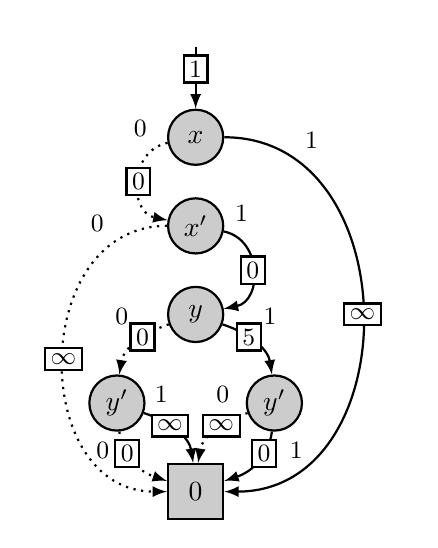
\begin{tikzpicture}[%
        costnode/.style={pos=0.6,rectangle,thick,solid,
                inner sep=2pt,draw,fill=white,text=black,font=\small},%
        decisionnode/.style={circle,thick,minimum size=4mm,
                inner sep=2pt,draw,fill=white!80!black,text=black,font=\normalsize},%
        xscale=2,yscale=1.5,>=latex]
    \node[] (before) at (0,3.85) {}; % incoming edge_value
    \node[decisionnode, minimum size=0.7cm] (x) at (0,3) {$x$};
    \node[decisionnode, minimum size=0.7cm] (xp) at (0,2.25) {$x'$};
    \node[decisionnode, minimum size=0.7cm] (y) at (0,1.5) {$y$};
    \node[decisionnode, minimum size=0.7cm] (yp0) at (-0.5,0.75) {$y'$};
    \node[decisionnode, minimum size=0.7cm] (yp1) at (0.5,0.75) {$y'$};
    \node[draw,thick,fill=white!80!black,rectangle, minimum size=0.7cm]
    (after0) at (0,0) {{$0$}};
    % % before
    \draw[->, thick] (before) to[bend right=0,label distance=0mm,edge
    label={},swap,pos=0.3] node[costnode,pos=0.35] {$1$} (x);
    % % x =>
    \draw[->, thick, dotted] (x) to[bend right=75,label distance=0mm,edge
    label={\small{$0$}},swap,pos=0.1] node[costnode,pos=0.5] {$0$} (xp);
    \draw[->, thick] (x) to[bend left=90,label distance=0mm,edge
    label={\small{$1$}},pos=0.15] node[costnode,pos=0.5] {$\infty$} (after0);
    % % xp =>
    \draw[->, thick, dotted] (xp) to[bend right=90,label distance=0mm,edge
    label={\small{$0$}},swap,pos=0.15] node[costnode,pos=0.5] {$\infty$} (after0);
    \draw[->, thick] (xp) to[bend left=75,label distance=0mm,edge
    label={\small{$1$}},pos=0.01] node[costnode,pos=0.5] {$0$} (y);
    % % y =>
    \draw[->, thick, dotted] (y) to[bend right=30,label distance=0mm,edge
    label={\small{$0$}\phantom{.}},swap,pos=0.3] node[costnode,pos=0.35] {$0$} (yp0);
    \draw[->, thick] (y) to[bend left=30,label distance=0mm,edge
    label={\phantom{.}\small{$1$}},pos=0.3] node[costnode,pos=0.35] {$5$} (yp1);
    % % yp0 =>
    \draw[->, thick, dotted] (yp0) to[bend right=30,label distance=0mm,edge
    label={\small{$0$}},swap,pos=0.01] node[costnode,pos=0.35] {$0$} (after0);
    \draw[->, thick] (yp0) to[bend left=30,label distance=0mm,edge
    label={\small{$1$}},pos=0.01] node[costnode,pos=0.35] {$\infty$} (after0);
    % % yp0 =>
    \draw[->, thick, dotted] (yp1) to[bend right=30,label distance=0mm,edge
    label={\small{$0$}\phantom{.}},swap,pos=0.01] node[costnode,pos=0.35] {$\infty$} (after0);
    \draw[->, thick] (yp1) to[bend left=30,label distance=0mm,edge
    label={\phantom{.}\small{$1$}},pos=0.01] node[costnode,pos=0.35] {$0$} (after0);
\end{tikzpicture}

        }
    }\hfill
    \subfloat[Two BDDs representing the transition relation of operator $o$, where the left BDD encodes the cost of 1 and the right BDD encodes the cost of 6.\label{fig:tr_bdds}]{
        \centering
        \makebox[0.5\textwidth][c]{
            
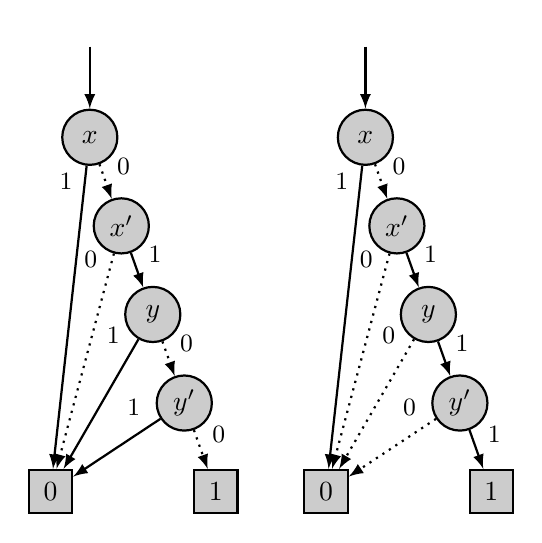
\begin{tikzpicture}[%
        costnode/.style={pos=0.6,rectangle,thick,solid,
                inner sep=2pt,draw,fill=white,text=black,font=\small},%
        decisionnode/.style={circle,thick,minimum size=4mm,
                inner sep=2pt,draw,fill=white!80!black,text=black,font=\normalsize},%
        xscale=2,yscale=1.5,>=latex]
    \begin{scope}
        \node[] (before) at (0,3.85) {}; % incoming edge_value
        \node[decisionnode, minimum size=0.7cm] (x) at (0,3) {$x$};
        \node[decisionnode, minimum size=0.7cm] (xp) at (0.2,2.25) {$x'$};
        \node[decisionnode, minimum size=0.7cm] (y) at (0.4,1.5) {$y$};
        \node[decisionnode, minimum size=0.7cm] (yp) at (0.6,0.75) {$y'$};
        \node[draw,thick,fill=white!80!black,rectangle, minimum size=0.55cm]
        (after0) at (-0.25,0) {{$0$}};
        \node[draw,thick,fill=white!80!black,rectangle, minimum size=0.55cm]
        (after1) at (0.8,0) {{$1$}};
        \draw[->, thick] (before) to (x);
        % x =>
        \draw[->, thick, dotted] (x) to[bend right=0,label distance=0mm,edge
        label={\small{$0$}},pos=0.6] (xp);
        \draw[->, thick] (x) to[bend left=0,label distance=0mm,edge
        label={\small{$1$}},swap,pos=0.1] (after0);
        % xp =>
        \draw[->, thick, dotted] (xp) to[bend right=0,label distance=0mm,edge
        label={\small{$0$}},swap,pos=0.1] (after0);
        \draw[->, thick] (xp) to[bend left=0,label distance=0mm,edge
        label={\small{$1$}},pos=0.6] (y);
        % y =>
        \draw[->, thick, dotted] (y) to[bend right=0,label distance=0mm,edge
        label={\small{$0$}},pos=0.6] (yp);
        \draw[->, thick] (y) to[bend left=0,label distance=0mm,edge
        label={\small{$1$}},swap,pos=0.1] (after0);
        % yp =>
        \draw[->, thick, dotted] (yp) to[bend right=0,label distance=0mm,edge
        label={\small{$0$}},pos=0.6] (after1);
        \draw[->, thick] (yp) to[bend left=0,label distance=0mm,edge
        label={\small{$1$}},swap,pos=0.1] (after0);
    \end{scope}
    \begin{scope}[xshift=1.75cm]
        \node[] (before) at (0,3.85) {}; % incoming edge_value
        \node[decisionnode, minimum size=0.7cm] (x) at (0,3) {$x$};
        \node[decisionnode, minimum size=0.7cm] (xp) at (0.2,2.25) {$x'$};
        \node[decisionnode, minimum size=0.7cm] (y) at (0.4,1.5) {$y$};
        \node[decisionnode, minimum size=0.7cm] (yp) at (0.6,0.75) {$y'$};
        \node[draw,thick,fill=white!80!black,rectangle, minimum size=0.55cm]
        (after0) at (-0.25,0) {{$0$}};
        \node[draw,thick,fill=white!80!black,rectangle, minimum size=0.55cm]
        (after1) at (0.8,0) {{$1$}};
        \draw[->, thick] (before) to (x);
        % x =>
        \draw[->, thick, dotted] (x) to[bend right=0,label distance=0mm,edge
        label={\small{$0$}},pos=0.6] (xp);
        \draw[->, thick] (x) to[bend left=0,label distance=0mm,edge
        label={\small{$1$}},swap,pos=0.1] (after0);
        % xp =>
        \draw[->, thick, dotted] (xp) to[bend right=0,label distance=0mm,edge
        label={\small{$0$}},swap,pos=0.1] (after0);
        \draw[->, thick] (xp) to[bend left=0,label distance=0mm,edge
        label={\small{$1$}},pos=0.6] (y);
        % y =>
        \draw[->, thick, dotted] (y) to[bend right=0,label distance=0mm,edge
        label={\small{$0$}},swap,pos=0.1] (after0);
        \draw[->, thick] (y) to[bend left=0,label distance=0mm,edge
        label={\small{$1$}},pos=0.6] (yp);
        % yp =>
        \draw[->, thick, dotted] (yp) to[bend right=0,label distance=0mm,edge
        label={\small{$0$}},swap,pos=0.1] (after0);
        \draw[->, thick] (yp) to[bend left=0,label distance=0mm,edge
        label={\small{$1$}},pos=0.6] (after1);
    \end{scope}
\end{tikzpicture}

        }
    }
    \caption[Visualization of symbolic representations of an operator with state-dependent action costs.]{Visualization of different variants for a symbolic representation of an operator $o = \langle \lnot x, x \rangle$ with state-dependent action costs $\costfun_o(s) = 5y +1$.}
    \label{fig:tr_sdac}
\end{figure}

\begin{example}
    Consider an operator $o = \langle \lnot x, x \rangle$ with sdac $\costfun_o(s) = 5y +1$ for $s \in \states$. \Cref{fig:tr_sdac} visualizes the transition relation of $o$ represented with different decision diagrams, where the precondition (predecessor states) are encoded with unprimed variables and the effects (successor states) with primed variables. \Cref{fig:tr_evmdd} represents the EVMDD representing the transition relation of $o$, while encoding the cost $\costfun_o(s)$ for each state $s \in \states$ at the same time. To represent the operator $o$ with BDDs, multiple BDDs are necessary to decompose the cost function.
    \Cref{fig:tr_bdds} illustrates two BDDs representing the two possible cost values of $\costfun_o(s)$, specifically 1 and 6. The left BDD encodes the cost of 1 by encoding $ \lnot y$ in the precondition.  Note that by adding the new precondition $\lnot y$, $\lnot y$ also holds in all successor states, i.e., $\lnot y'$, since variable $y$ does not occur in the effect (closed world assumption). Similarly, the right BDD encodes $y$ as a precondition to obtain a cost of 6.
\end{example}

\paragraph{Empirical Evaluation.}  While \textcite{speck-et-al-icaps2018}  reported results comparing symbolic search with EVMDDs and translation-based approaches, here we present new empirical results incorporating recent advances, planners, and benchmarks for planning with sdac \autocite{geisser-phd2018,corraya-et-al-ki2019,speck-et-al-icaps2021}.

\Cref{tab:coverage_sdac} shows the coverage (number of optimally solved instances) of explicit \astar{} search \autocite{hart-et-al-ieeessc1968} with various translation-based heuristics \autocite{geisser-phd2018} and forward, backward and bidirectional symbolic search with all data structures represented as either EVMDDs \autocite{speck-et-al-icaps2018} or BDDs.
In explicit \astar{} search for planning with sdac, the cost function is represented as an EVMDD, which is used to evaluate the actual costs ($g$-values) \autocite{geisser-phd2018}.
We consider the \heu{blind}{} heuristic and the \heu{max}{} heuristic \autocite{bonet-geffner-ecp1999}, which is analyzed in two versions: \heu{max}{c} uses the combinatorial translation \autocite{geisser-phd2018} and \heu{max}{dd} uses the EVMDD translation \autocite{geisser-et-al-ijcai2015} to compute the heuristic values.

\begin{table}
    \begin{center}
        \resizebox{1\textwidth}{!}{
            \newcommand{\numtasks}[1]{(#1)}
\begin{tabular}{@{}lrrrrrrrrr@{}}
    \toprule
    Algorithm & \multicolumn{3}{c}{\astar{} (explicit)} & \multicolumn{3}{c}{\textbf{EVMDD Search}} & \multicolumn{3}{c}{\textbf{BDD Search}} \\
    \cmidrule(lr){2-4} \cmidrule(lr){5-7} \cmidrule(lr){8-10}
    Domain (\# Tasks) & \heu{blind}{} & \heu{max}{c} & \heu{max}{dd} & fwd & bwd & bid & fwd & bwd & bid \\
    \midrule
    Asterix \numtasks{30} & 10 & 5 & 10 & \textbf{30} & 29 & \textbf{30} & \textbf{30} & 28 & \textbf{30} \\
    
    Pegsol \numtasks{100} & \textbf{96} & 0 & \textbf{96} & 86 & 16 & 88 & \textbf{96} & 23 & \textbf{96} \\
    % Greedy Pegsol \numtasks{50} & 48 & 0 & 48 & 44 & 8 & 44 & 48 & 14 & 48 \\
    % Greedy Pegsol2 \numtasks{50} & 48 & 0 & 48 & 42 & 8 & 44 & 48 & 9 & 48 \\
    % Greedy Pegsol-08 \numtasks{30} & \textbf{29} & 0 & \textbf{29} & 27 & 7 & 27 & \textbf{29} & 12 & \textbf{29} \\
    % Greedy Pegsol-11 \numtasks{20} & \textbf{19} & 0 & \textbf{19} & 17 & 1 & 17 & \textbf{19} & 2 & \textbf{19} \\
    % Greedy Pegsol-08-v2 \numtasks{30} & \textbf{29} & 0 & \textbf{29} & 26 & 7 & 27 & \textbf{29} & 8 & \textbf{29} \\
    % Greedy Pegsol-11-v2 \numtasks{20} & \textbf{19} & 0 & \textbf{19} & 16 & 1 & 17 & \textbf{19} & 1 & \textbf{19} \\

    Gripper \numtasks{30} & 8 & 4 & 8 & 11 & 8 & 12 & \textbf{20} & 14 & 19 \\

    PSR Large \numtasks{100} & 33 & 12 & \textbf{39} & 36 & 20 & 36 & 28 & 23 & 28 \\
    PSR Middle \numtasks{100} & 79 &  34 & 84 & 88 & 55 & \textbf{90} & 74 & 58 & 74 \\
    %PSR Large \numtasks{50} & 20 & 11 & \textbf{23} & 21 & 13 & 22 & 18 & 15 & 18 \\
    %PSR Large Full \numtasks{50} & 13 & 1 & \textbf{16} & 15 & 7 & 14 & 10 & 8 & 10 \\
    % PSR Middle \numtasks{50} & 48 & 26 & 49 & \textbf{50} & 37 & \textbf{50} & 43 & 37 & 43 \\
    % PSR Middle Full \numtasks{50} & 31 & 8 & 35 & 38 & 18 & \textbf{40} & 31 & 21 & 31 \\

    Openstacks \numtasks{70} & 9 & 10 & 10 & 40 & 30 &  38 & \textbf{54} & 46 & 51 \\
    % Openstacks-08 \numtasks{30} & 6 & 6 & 6 & 14 & 12 & 12 & \textbf{18} & 15 & \textbf{18} \\
    % Openstacks-11 \numtasks{20} & 3 & 4 & 4 & \textbf{20} & 15 & \textbf{20} & \textbf{20} & \textbf{20} & \textbf{20} \\
    % Openstacks-14 \numtasks{20} & 0 & 0 & 0 & 6 & 3 & 6 & \textbf{16} & 11 & 13 \\

    Transport \numtasks{30} & 24 & 19 & 24 & 24 & 23 & \textbf{29} & 24 & 23 & 28 \\
    TSP \numtasks{26} & \textbf{21} & 12 & \textbf{21} & 15 & 10 & 13 & 18 & 10 & 18 \\
    \midrule
    \textbf{Sum \numtasks{486}} & 280 & 96 & 292 & 330 & 191 & 336 & \textbf{344} & 225 & \textbf{344} \\
    \bottomrule
    \end{tabular}
    
        }
    \end{center}
    \caption[Coverage for planning with state-dependent action costs.]{Coverage (number of optimally solved instances) for explicit and symbolic search algorithms on versions of planning domains with state-dependent action costs.}
    \label{tab:coverage_sdac}
\end{table}

\bigskip
Overall, it can be seen that native support for sdac within symbolic search compares favorably with explicit search approaches.
%Symbolic (bidirectional) search based on EVMDDs or BDDs solves most tasks overall. 
Comparing symbolic search with BDDs and EVMDDs, there are domain-wise differences in coverage, with BDD-based symbolic search performing best overall.
However, the structural advantages of EVMDDs pay off especially in the PSR domain, where the cost function is complex and contains derived variables represented with the symbolic translation described in \Cref{ch:axioms}.\footnote{In \Cref{sec:combination}, the relationship and interplay of the different planning extensions is discussed in more detail.} Looking at the explicit approaches, we can see that in many domains it is not possible to perform a combinatorial translation \heu{max}{c}, which often requires exponentially many operators and thus solves the least number of tasks.
Explicit \astar{} search with the $\heu{blind}{}$ and the $\heu{max}{dd}$ heuristics performs much better.
These configurations use EVMDDs to concisely represent the cost functions and as a basis for the heuristic computation, which seems to pay off.
It turns out that the heuristic estimates of $\heu{max}{dd}$ can help the search, but the performance of $\heu{max}{dd}$ is still often not comparable to symbolic blind search.
However, there are domains where explicit heuristic search performs better than symbolic search. This shows that, similar to classical planning, a potential portfolio planner of these complementary search strategies could lead to a state-of-the-art planner that combines both strengths \autocite{sievers-et-al-aaai2019}.

%\todo{links to planners and benchmarks}
%\section{Empirical Evaluation}


%\section{Summary}
